% This is the Reed College LaTeX thesis template. Most of the work 
% for the document class was done by Sam Noble (SN), as well as this
% template. Later comments etc. by Ben Salzberg (BTS). Additional
% restructuring and APA support by Jess Youngberg (JY).
% Your comments and suggestions are more than welcome; please email
% them to cus@reed.edu
%
% See http://web.reed.edu/cis/help/latex.html for help. There are a 
% great bunch of help pages there, with notes on
% getting started, bibtex, etc. Go there and read it if you're not
% already familiar with LaTeX.
%
% Any line that starts with a percent symbol is a comment. 
% They won't show up in the document, and are useful for notes 
% to yourself and explaining commands. 
% Commenting also removes a line from the document; 
% very handy for troubleshooting problems. -BTS

% As far as I know, this follows the requirements laid out in 
% the 2002-2003 Senior Handbook. Ask a librarian to check the 
% document before binding. -SN

%%
%% Preamble
%%
% \documentclass{<something>} must begin each LaTeX document
\documentclass[12pt,twoside]{reedthesis}
% Packages are extensions to the basic LaTeX functions. Whatever you
% want to typeset, there is probably a package out there for it.
% Chemistry (chemtex), screenplays, you name it.
% Check out CTAN to see: http://www.ctan.org/
%%
\usepackage{graphicx,latexsym} 
\usepackage{amssymb,amsthm,amsmath}
\usepackage{longtable,booktabs,setspace} 
\usepackage{chemarr} %% Useful for one reaction arrow, useless if you're not a chem major
\usepackage[hyphens]{url}
\usepackage{rotating}
\usepackage{natbib}
% Comment out the natbib line above and uncomment the following two lines to use the new 
% biblatex-chicago style, for Chicago A. Also make some changes at the end where the 
% bibliography is included. 
%\usepackage{biblatex-chicago}
%\bibliography{thesis}


%here are packages and other things that I, Nick, have added:
\usepackage{algorithm}
\usepackage[noend]{algpseudocode}
\usepackage{amsthm} % package for proof environment

\newenvironment{blockquote}{%
  \par%
  \medskip
  \leftskip=4em\rightskip=2em%
  \noindent\ignorespaces}{%
  \par\medskip}


% \usepackage{times} % other fonts are available like times, bookman, charter, palatino

\title{My Final College Paper}
\author{Your R. Name}
% The month and year that you submit your FINAL draft TO THE LIBRARY (May or December)
\date{May 200x}
\division{Mathematics and Natural Sciences}
\advisor{Advisor F. Name}
%If you have two advisors for some reason, you can use the following
%\altadvisor{Your Other Advisor}
%%% Remember to use the correct department!
\department{Mathematics}
% if you're writing a thesis in an interdisciplinary major,
% uncomment the line below and change the text as appropriate.
% check the Senior Handbook if unsure.
%\thedivisionof{The Established Interdisciplinary Committee for}
% if you want the approval page to say "Approved for the Committee",
% uncomment the next line
%\approvedforthe{Committee}

\setlength{\parskip}{0pt}
%%
%% End Preamble
%%
%% The fun begins:
\begin{document}

  \maketitle
  \frontmatter % this stuff will be roman-numbered
  \pagestyle{empty} % this removes page numbers from the frontmatter

% Acknowledgements (Acceptable American spelling) are optional
% So are Acknowledgments (proper English spelling)
    \chapter*{Acknowledgements}
	I want to thank a few people.

% The preface is optional
% To remove it, comment it out or delete it.
    \chapter*{Preface}
	This is an example of a thesis setup to use the reed thesis document class.
	
	

    \chapter*{List of Abbreviations}
		You can always change the way your abbreviations are formatted. Play around with it yourself, use tables, or come to CUS if you'd like to change the way it looks. You can also completely remove this chapter if you have no need for a list of abbreviations. Here is an example of what this could look like:

	\begin{table}[h]
	\centering % You could remove this to move table to the left
	\begin{tabular}{ll}
		\textbf{ABC}  	&  American Broadcasting Company \\
		\textbf{CBS}  	&  Columbia Broadcasting System\\
		\textbf{CDC}  	&  Center for Disease Control \\
		\textbf{CIA}  	&  Central Intelligence Agency\\
		\textbf{CLBR} 	&  Center for Life Beyond Reed\\
		\textbf{CUS}  	&  Computer User Services\\
		\textbf{FBI}  	&  Federal Bureau of Investigation\\
		\textbf{NBC}  	&  National Broadcasting Corporation\\
	\end{tabular}
	\end{table}
	

    \tableofcontents
% if you want a list of tables, optional
    \listoftables
% if you want a list of figures, also optional
    \listoffigures

% The abstract is not required if you're writing a creative thesis (but aren't they all?)
% If your abstract is longer than a page, there may be a formatting issue.
    \chapter*{Abstract}
	The preface pretty much says it all.
	
	\chapter*{Dedication}
	You can have a dedication here if you wish.

  \mainmatter % here the regular arabic numbering starts
  \pagestyle{fancyplain} % turns page numbering back on

%The \introduction command is provided as a convenience.
%if you want special chapter formatting, you'll probably want to avoid using it altogether

    \chapter*{Introduction}
         \addcontentsline{toc}{chapter}{Introduction}
	\chaptermark{Introduction}
	\markboth{Introduction}{Introduction}
	% The three lines above are to make sure that the headers are right, that the intro gets included in the table of contents, and that it doesn't get numbered 1 so that chapter one is 1.

% Double spacing: if you want to double space, or one and a half 
% space, uncomment one of the following lines. You can go back to 
% single spacing with the \singlespacing command.
% \onehalfspacing
% \doublespacing

\marginpar{I keep wanting to revise the order of the sections since they all sort of play into each other}


\section{Forward}
\marginpar{not sure if it's appropriate to have this here? I expect it to be a short explanation of my expository style.}
This is an interdisciplinary thesis that combines Computer Science and Biology. In this background chapter I have written sections designed to make the computer science more accessible to the biologists, sections designed to make the biology more accessible to the computer scientists, and hopefully in tandem these sections will make everything a bit more accessible to the reader who knows neither. For this reason, information presented in my background chapter may oscillate between trivially familiar and dauntingly foreign, depending on each reader's varying base of knowledge. So feel free to read up on the additional resources I present if you're not comfortable with the foundational concepts, or to skip around if you already know what I'm talking about.

\section{Graph Theory in Systems Biology}
%Briefly define Systems Biology
Systems biology is a modern, holistic, modeling-focused approach to the study of life. \par

%Briefly talk about what a protein is, how cells use them to do basically everything
Biologically speaking, this thesis is primarily concerned with modeling how proteins interact. But in order to understand why protein interactions are important, it's important to have some context about how cells work. So if you're not familiar with the biological side of things, consider this a small primer. Most of what you need to know is encapsulated in a rule of thumb called the Central Dogma of Biology. My explanation of this rule will contextualize what proteins are, what they do, and why they're important. But to do that we have to start with DNA. The Central Dogma of Biology states that information in the cell flows in a stream from DNA to RNA to protein (in general)\footnote{For almost every rule in biology there is at least one exception. This is even true of the Central Dogma. For example, there are viruses who encode information in RNA and use a special enzyme to transfer that information to DNA when they infect a host. But in almost every organism, we observe that the Central Dogma holds true.}. DNA, DeoxyriboNucleic Acid, is a molecule that can be arranged into long chains called polymers. The individual links of the chains, the subunits of the polymer, consist of a sugar backbone and a modular base. The base can be Adenine, Thymine, Cytosine, or Guanine (shortened A T C or G), and various cellular apparatuses can distinguish between these bases. Just like a computer uses sequences of bits in memory to encode numbers, a cell uses sequences of bases on DNA polymers to encode information. In fact, it's reasonable to think about the DNA in a cell like the memory in a computer: slow-access, long-term information storage. The DNA is where the cell stores recipes (called genes) for making tools that it uses to take actions. That may sound weirdly generalized, but that's because the concept is very general. Basically everything a cell does - grow, divide, absorb energy, synthesize compounds, respond to stimuli, etc. - is encoded in its DNA. But this is not the whole story. Encoding something into DNA does not instantly make it so. Instead, the functions encoded in DNA must be executed by the cellular system in order to take effect. The next piece of the Central Dogma, RNA, is a major part of how this execution occurs. \par
	
	RNA, RiboNucleic Acid, is a molecule similar to DNA. Like DNA, it can be arranged into long chains called polymers. Like DNA, each subunit in the RNA polymer consists of a sugar backbone and a modular base. Like DNA, there are four possible modular bases which are used in sequence to encode information. Indeed, RNA is quite similar to DNA, in fact their molecular structures only differ by the presence or absence of a single Oxygen atom. But the \textit{function} of RNA in the cell is distinct. If the DNA in a cell is like the memory of a computer, then the RNA in a cell is kind of like the RAM: quick-access, short-term information storage. DNA stores recipes for making tools, but in order to actually use them, the cell first \textbf{transcribes}\footnote{Transcription is an important key word that refers specifically to the synthesis of an RNA polymer from a gene in the DNA.} the recipe into RNA form. To do this, the cell reads the information off of a gene in the DNA and creates a short and portable RNA polymer that encodes the same\footnote{In reality, this is sort of an oversimplification. Things like post-transcriptional modification (e.g. pre-mRNA splicing) often cause a piece of mRNA to have information content that differs from the gene from which it was transcribed. But the less biologically inclined reader need not concern themselves with this detail if their goal is to develop a cursory understanding of the Central Dogma.} information. This polymer is called a messenger\footnote{We make this distinction because there are other functions fulfilled by RNA in the cell, but for the purposes of this thesis a less biologically inclined reader need not know them. For a cursory working understanding of the Central Dogma, it is sufficient to focus on messenger RNA.} RNA (mRNA). The utility of using mRNA to convey information is manifold. In particular, it allows the cell to relay information to distal parts of itself while keeping the DNA sequestered in a secure location: mRNA copies of genes are free to move about the cell without the risk of damaging the master copy contained in the DNA. Additionally, by transcribing the same gene multiple times multiple mRNA copies can be made. This makes the information encoded in the gene accessible to multiple pieces of cellular apparatus at a time which greatly increases the speed of information propagation. This is important when the cell needs a widespread effect to occur quickly. So the purpose of DNA is long term information storage, and the purpose of RNA is quick, widespread propagation of the information in the DNA. The third piece of the Central Dogma, protein, is how the cell uses the information to perform actions. \par

	Proteins 

%Talk about some important findings in the biochemical literature (ideally relevant to some dataset(s) that I use later on in the thesis), leading into how we have a vast amount of findings about individual proteins and small scale protein interaction data

%talk about how proteins interact with each other on a vast scale (maybe show one of those huge interactome visualization images)

%present a graph as a tool for visualization and inference on this vast dataset

\subsection{Graphs and Graph Algorithms}
\marginpar{not 100\% sure that this needs to be its own subsection. The main argument in favor of it for me is that it might be nice to have a clearly delineated place where a reader can find the definition of a graph. I guess I'll see how big it is when I write it up and figure it out based on that.}
\begin{itemize}
\item rigorously define what a graph is (probably include some snazzy figures to demonstrate)
\item present some graph algorithms, their applications in the context of systems biology
\end{itemize}


\section{Hypergraphs}


\section{A Crash Course in P Versus NP}	
\indent Any currently discovered algorithm that we might refer to as 'efficient' is in a class called P. P stands for Polynomial time. Members of the class P can be solved in a number of timesteps that is a polynomial of the size of the input. For example, if I had a list of length $n$ and I wanted to write that list in reverse order, an algorithm to do that might look something like this:
\begin{algorithm}
\caption{Write a List $ls$ in Reverse Order}
\begin{algorithmic} 
\State $newList$ $\gets$ [ ]
\State $i\gets$ length($ls$)$-1$
\While{$i \geq 0$}
\State append $ls[i]$ to $newList$
\State $i \gets i - 1$
\EndWhile
\State return $newList$
\end{algorithmic}
\end{algorithm}
    
\marginpar{not exactly certain where I want to put a definition of Big O notation. It feels like it would be awkward to put it right here in the middle of explaining what P is, but doing it before talking about time complexity feels like I'm giving the reader a bunch of information that they have no reason to care about yet. Maybe I'll put it in an appendix and simply reference it?}    This algorithm would have time complexity $O(n)$ since it would take one timestep to write down each element of the list and the rest of the operations do not scale with the size of the input\footnote{When describing the runtime of an algorithm, it is conventional and generally useful to talk about its Asymptotic Time Complexity instead of its exact time complexity. Basically, this means we only worry about additional timesteps in the algorithm when they scale with the size of the input.}. The number $n$ is in fact a polynomial of the number $n$, so this problem can be solved in polynomial time. It is in the class P. To give another example, if I had a list of length $n$ and I wanted to make a table out of it with a row of $n$ zeros for each entry of the list, the algorithm might look something like this:
\begin{algorithm}
\caption{Write a Table with a Row of Zeros for Each Entry in a List $ls$}
\begin{algorithmic}
\State $table$ $\gets$ [ ]
\For {each item in $ls$}
\State append an empty list to $table$
\For {each item in $ls$}
\State append 0 to the newly created list
\EndFor
\EndFor
\State return $table$
\end{algorithmic}
\end{algorithm}
\marginpar{I don't know why this paragraph gets cut in half by the algorithm but the text is definitely below the algorithm in the .TeX file so ???}
	This algorithm has time complexity $O(n^2)$ since for each element in the $n$ sized list, we write down $n$ new table entries (and the sum of $n$ groups of $n$ is $n^2$), and the other operations don't scale with the size of the input. Similarly to the case above, we observe that $n^2$ is a polynomial of $n$. Therefore this task can be accomplished in polynomial time and the problem of creating an $n$ by $n$ is in the class P.\par
\marginpar{I kind of wanted to rereference the footnote from the above paragraph here, but I couldn't figure out how to do that. The solutions I found on stack exchange didn't seem to work.}

There exists another class of problems called NP, which stands for Nondeterministic Polynomial time. These are problems that can be computed in polynomial time by a theoretical construct called a nondeterministic Turing machine,\footnote{PLACEHOLDER reference for reading up on nondeterminism} or equivalently\footnote{PLACEHOLDER reference to proof showing that the nondeterminism definition and witness definition are equivalent} (and for the purposes of this introduction, more expediently), questions for which we can determine whether a putative solution is correct in polynomial time. Since every problem in P can be \textit{solved} in polynomial time by definition, we can infer that every problem in P is also in NP. But importantly, NP also contains problems which appear\footnote{Currently there is no proof which says whether or not P and NP are equivalent, but the hardest problems in NP have remained robustly intractable for quite a long time. Thus it \textit{appears} that some problems in NP are not in P.} to not be solvable in polynomial time. These apparently intractable problems are in a subset of NP called NP-Complete, which refers to problems that are in NP (i.e. we can determine whether a putative solution is correct in polynomial time), and are NP-hard\footnote{If you're new to this terminology and this term feels poorly defined, don't worry. I explain the basis of NP-hardness and NP-Completeness in more detail later on. For now just follow the example.}, which means they are at least as hard as the hardest problems in NP. An example of a member of NP-Complete is the Subset Sum problem, which asks:
\begin{blockquote}
For a set of numbers S, is there a non-empty subset of those numbers that sums to zero?
\end{blockquote}
To show that this is a member of NP, I will give a polynomial time algorithm that verifies whether a putative answer is correct. For this problem, that means simply checking whether the candidate subset sums to zero.

\begin{algorithm}
\caption{Verify a Putative Answer for Subset Sum}
\begin{algorithmic}
\State $total \gets 0$
\For{each number $n$ in the given subset}
\State $total \gets total + n$
\EndFor
\If{$total = 0$}
\State return True
\Else
\State return False
\EndIf
\end{algorithmic}
\end{algorithm}

As you can see, this algorithm simply traverses the subset once, totaling up the values and returning True if they sum to zero and False otherwise. Since we look at each value in the subset once and the rest of the operations do not scale with the input size, this algorithm has time complexity $O(n)$. And of course, $n$ is a polynomial of the input size $n$. So by the definition given above, Subset Sum is in NP. But the simplicity of the verifying algorithm can be deceptive. Don't be fooled. Subset Sum doesn't seem daunting at first, but a naive implementation of an algorithm to solve it requires checking every subset of S:  
\begin{algorithm}
\caption{Subset Sum of a Set S}
\begin{algorithmic}
\For{each subset of S}
\State compute the sum of that subset
\If{the sum is 0}
\State return True
\EndIf
\EndFor
\State return False
\end{algorithmic}
\end{algorithm}

This algorithm computes the sum of every subset in S in order to see if any of them sum to zero. Since there are $2^{|S|}$ subsets of S, this algorithm has a time complexity of $O(2^n)$, which is \textit{very} slow, and I'll give an estimate of just how slow it is using real world figures a little bit later on. But there are plenty of algorithms that have terrible runtimes if implemented poorly, and plenty of algorithms whose fastest known implementation is better than one might expect given the problem they are designed to solve. What makes us think that a polynomial time algorithm for Subset Sum simply hasn't been discovered yet? The answer is complicated. It is possible that there is a polynomial time algorithm for Subset Sum. There is no discovered proof that rules out this scenario. But the discovery of a polynomial time algorithm that solves Subset Sum would have profound implications and would cause an upheaval in Complexity Theory as we currently know it. I'll explain why. \par
	There is a proof \marginpar{Find a reference for proof: 3-SAT reduces to Subset Sum} which demonstrates (using a method called reduction) that if we could solve Subset Sum in polynomial time, then we could solve another problem called 3-SAT in polynomial time. This problem, 3-SAT (short for 3 Conjunctive Normal Form Boolean Satisfiability), is readily convertible to a more general problem called SAT (short for Boolean Satisfiability), which is a very important problem in Complexity Theory. A foundational work called the Cook-Levin theorem \marginpar{Reference the Cook-Levin Theorem} proves that SAT is NP-Complete. In other words:
\begin{enumerate}
\item SAT is in the class NP
\item \textbf{Any} problem in the class NP can be reduced in polynomial time to a SAT problem
\end{enumerate}
The implications of this proof are profound. Fact \textbf{2} means that if we can do SAT efficiently, then in polynomial time we can convert any problem in NP to a SAT problem and solve it using our efficient SAT solving method. Thus if we could do SAT efficiently, we could do any problem in NP efficiently as well. More formally, if we had a polynomial time algorithm for SAT, we could convert any problem in NP to a SAT problem in polynomial time, and then solve that SAT problem in polynomial time. A polynomial $+$ a polynomial $=$ another polynomial, so the time complexity of this solution method would be polynomial. Thus, if we had a polynomial time algorithm for SAT, not only would SAT be a member of P, but (by the Cook-Levin theorem) \textbf{\textit{every}} member of NP would be a member of P. Expressed compactly:
\begin{center}
$\exists$ a polynomial time algorithm which solves SAT $\implies$ P = NP
\end{center}

Now let's connect this observation with Subset Sum. As I stated above, there is a proof which demonstrates that if we could solve Subset Sum in polynomial time, then we could solve a problem called 3-SAT in polynomial time. In other words, we can convert any 3-SAT problem to a Subset Sum problem in polynomial time. Further, a 3-SAT problem can be converted to a SAT problem in polynomial time. Thus if we wanted to solve any SAT problem, we could follow this algorithm:

\begin{algorithm}
\caption{Solve a SAT problem $S$ via Subset Sum}
\begin{algorithmic}
\State Given a SAT problem $S$, convert the problem to a 3-SAT problem, name it $T$
\State convert $T$ to a Subset Sum problem, name it $U$
\State solve $U$ using a Subset Sum solving algorithm
\State return the result of solving $U$
\end{algorithmic}
\end{algorithm}

Thus if we had a polynomial time algorithm for solving Subset Sum, all the pieces of this algorithm would take only polynomial time. And therefore we would have a polynomial time algorithm for solving SAT. Therefore by the Cook-Levin theorem P would equal NP. What I am describing is the basis of NP-hardness, the concept I glossed over earlier. NP-hardness is a generalized version of Fact \textbf{2} from the Cook-Levin theorem: a problem is NP-hard if any problem in the class NP can be reduced to an instance of that problem in polynomial time. In order to demonstrate that SAT is NP-hard, the Cook-Levin theorem had to do a lot of heavy lifting (e.g. reasoning about what it is \textit{possible} for a nondeterministic Turing machine to do), but because we know that SAT is NP-hard, proving that other problems are NP-hard becomes much easier. We simply show that any instance of SAT can be reduced to an instance of the problem in question, and constructing an algorithm similar to the one shown above demonstrates that the problem in question is NP-hard. Any problem that is in NP and is NP-hard we call NP-Complete. \par

With NP-Completeness explained more extensively, we can begin to understand why the discovery of a polynomial time algorithm for Subset Sum would cause an upheaval in Complexity Theory as we know it, why we might expect Subset Sum (and all other members of the class NP-Complete) to be robustly inefficient. And any mathematician readers are going to have to forgive me for a moment because in the absence of a proof I'm going to have to use somewhat empirical ideas to explain this expectation. The question of whether NP-Complete problems can be solved in polynomial time (equivalently, the question of whether P is equal to NP) is widely considered the most important open question in computer science today. Formally introduced in 1971,\marginpar{cite Cook, Stephen (1971). "The complexity of theorem proving procedures". Proceedings of the Third Annual ACM Symposium on Theory of Computing. pp. 151–158.} the problem has remained open for quite some time now, despite a million dollar bounty on its head courtesy of the Clay Mathematics Institute. Any polynomial time algorithm for \textbf{any} NP-Complete problem (of which there are many many examples \marginpar{tempted to cite the website that we saw at the end of C\&C but I couldn't find it by googling}) would demonstrate that P = NP, but none have arisen in the 46 years since the description of the problem. Indeed, the fact that proving P=NP simply requires an example of an algorithm for an NP-Complete problem that runs in polynomial time makes it seem like the positive direction of the proof is somehow easier than the negative. It seems that since the method of a whole family of feasible proofs is obvious, if the positive direction were correct it seems more likely that we would have found it by now. The negative direction on the other hand is quite murky. How does one even begin to prove that P $\neq$ NP? Complexity theorists are for the most part just as baffled as you are for this particular question\marginpar{should probably find some citation of a published paper that disproves a possible candidate proof method for showing P $\neq$ NP}. For this reason and a few other empirical observations about the current state of Complexity Theory\marginpar{maybe cite that blogpost from C\&C? Or some papers that that blogpost cites?}, our \textit{expectation} is that P $\neq$ NP and therefore we expect that Subset Sum and Hypergraph Shortest Path do not have polynomial time algorithms. That expectation cannot be said to be \textit{correct} until a proof arises, but in the absence of a proof we are stuck with algorithms that run in super-polynomial time. But just how bad is super-polynomial time complexity? I'll explain in concrete terms below.


	All of the biologically applicable standard graph algorithms we discussed earlier (e.g. finding the shortest path from a start node to each other node, finding the strongly connected components in a directed graph, breadth first search) \marginpar{these examples are subject to change, will clean them up when I write the 'biological applications of graph theory' section of the intro} run in polynomial time. Computers can do them reasonably quickly, even on graphs of substantial size that we might encounter in the real world (e.g. a graph depicting components of a bunch of signaling pathways, a graph depicting who is friends with who on a social network, a graph depicting actors who have worked with other actors in films). The qualified attribute "reasonably quickly" means that if your graph is big enough and your algorithm's time complexity is slow enough (e.g. $O(n^3)$ or $O(n^2)$ instead of $O(n \cdot \log n)$ or $O(n)$), you might have to buy some computation from Amazon, but it will get done.\par This is not true of any known algorithm that computes the solution to an NP-hard problem for all inputs (e.g. an algorithm that solves Subset Sum, an algorithm that solves Hypergraph Shortest Path). These algorithms run \textit{unreasonably} slowly. That is to say, if the input graph is big enough, you can buy as much computation from Amazon as you want - the algorithm still might not be finished for years (and often much longer!). These algorithms have time complexity that is worse than polynomial with respect to the size of the input. A common and reasonable example of a super-polynomial time complexity is $2^n$. This time complexity is common because $2^n$ is the number of timesteps it takes to make each possible set of binary choices for a set of $n$ decisions, which is something you might often need to do to tackle a difficult problem. To convey an understanding of just how bad this is, I'll provide a hypothetical example using charitable, seat-of-the-pants calculations conducted using concrete figures from the real world:

\begin{blockquote}
At time of writing, the highest clock speed (i.e. the rate at which a processor does an operation) offered from Amazon's cloud computing services is 3.3 gigahertz. In other words, the processor does something $3.3 \cdot 10^9$ times per second. That's pretty fast, and even though in the real world the processor is never devoting all of those ticks to one particular process, for this example let's be charitable and say that all of the ticks go directly towards running the algorithm. For $n = 100$, so for example that could be a graph with 100 nodes, a rough estimate of runtime an algorithm with time complexity $n^2$ would take $\frac{100^2}{3.3 \cdot 10^9} = 3.03$ microseconds, which Wolfram Alpha informs me is roughly twice the half-life of a muon (whatever that is, the point is it's very quick). For the same $n$, a rough estimate of the runtime of an algorithm with time complexity $2^n$ would take $\frac{2^{100}}{3.3 \cdot 10^9} = 1.217 \cdot 10^{13}$ average Gregorian years, approximately \textbf{880 times the age of the universe}. And just to show that processing power isn't the problem, consider that even if we bought one hundred 3.3 GHz computers to run the problem concurrently, we're still looking at a computation time of roughly \textbf{9 times the age of the universe}. Clearly, this is a prohibitively expensive computation.
\end{blockquote}

\section{Parameterized Complexity: Practical Solutions to Theoretically Impossible Problems}

\section{Why use it?}
	
\LaTeX\ does a great job of formatting tables and paragraphs. Its line-breaking algorithm was the subject of a PhD.\thinspace thesis. It does a fine job of automatically inserting ligatures, and to top it all off it is the only way to typeset good-looking mathematics.

\section{Who should use it?}

Anyone who needs to use math, tables, a lot of figures, complex cross-references, IPA or who just cares about the final appearance of their document should use \LaTeX. At Reed, math majors are required to use it, most physics majors will want to use it, and many other science majors may want it also.
	
    \chapter{The First}
    	This is the first page of the first chapter. You may delete the contents of this chapter so you can add your own text; it's just here to show you some examples. 
	
\section{References, Labels, Custom Commands and Footnotes}
It is easy to refer to anything within your document using the \texttt{label} and \texttt{ref} tags.  Labels must be unique and shouldn't use any odd characters; generally sticking to letters and numbers (no spaces) should be fine. Put the label on whatever you want to refer to, and put the reference where you want the reference. \LaTeX\ will keep track of the chapter, section, and figure or table numbers for you. 

\subsection{References and Labels}
Sometimes you'd like to refer to a table or figure, e.g. you can see in Figure \ref{subd2} that you can rotate figures . Start by labeling your figure or table with the label command (\verb=\label{labelvariable}=) below the caption (see the chapter on graphics and tables for examples). Then when you would like to refer to the table or figure, use the ref command (\verb=\ref{labelvariable}=). Make sure your label variables are unique; you can't have two elements named ``default." Also, since the reference command only puts the figure or table number, you will have to put  ``Table" or ``Figure" as appropriate, as seen in the following examples:

 As I showed in Table \ref{inheritance} many factors can be assumed to follow from inheritance. Also see the Figure \ref{subd} for an illustration.
 
\subsection{Custom Commands}\label{commands}
Are you sick of writing the same complex equation or phrase over and over? 

The custom commands should be placed in the preamble, or at least prior to the first usage of the command. The structure of the \verb=\newcommand= consists of the name of the new command in curly braces, the number of arguments to be made in square brackets and then, inside a new set of curly braces, the command(s) that make up the new command. The whole thing is sandwiched inside a larger set of curly braces. 

% Note: you cannot use numbers in your commands!
\newcommand{\hydro}{H$_2$SO$_4$}

In other words, if you want to make a shorthand for H$_2$SO$_4$, which doesn't include an argument, you would write: \verb=\newcommand{\hydro}{H$_2$SO$_4$}= and then when you needed  to use the command you would type \verb=\hydro=. (sans verb and the equals sign brackets, if you're looking at the .tex version). For example: \hydro

\subsection{Footnotes and Endnotes}
	You might want to footnote something.\footnote{footnote text} Be sure to leave no spaces between the word immediately preceding the footnote command and the command itself. The footnote will be in a smaller font and placed appropriately. Endnotes work in much the same way. More information can be found about both on the CUS site.
	
\section{Bibliographies}
	Of course you will need to cite things, and you will probably accumulate an armful of sources. This is why BibTeX was created. For more information about BibTeX and bibliographies, see our CUS site (\url{web.reed.edu/cis/help/latex/index.html})\footnote{\cite{reedweb:2007}}. There are three pages on this topic: {\it bibtex} (which talks about using BibTeX, at \url{/latex/bibtex.html}), {\it bibtexstyles} (about how to find and use the bibliography style that best suits your needs, at \url{/latex/bibtexstyles.html}) and {\it bibman} (which covers how to make and maintain a bibliography by hand, without BibTeX, at at \url{/latex/bibman.html}). The last page will not be useful unless you have only a few sources. There used to be APA stuff here, but we don't need it since I've fixed this with my apa-good natbib style file.
	
\subsection{Tips for Bibliographies}
\begin{enumerate}
\item Like with thesis formatting, the sooner you start compiling your bibliography for something as large as thesis, the better. Typing in source after source is mind-numbing enough; do you really want to do it for hours on end in late April? Think of it as procrastination.
\item The cite key (a citation's label) needs to be unique from the other entries.
\item When you have more than one author or editor, you need to separate each author's name by the word ``and'' e.g.\\ \verb+Author = {Noble, Sam and Youngberg, Jessica},+.
\item Bibliographies made using BibTeX (whether manually or using a manager) accept LaTeX markup, so you can italicize and add symbols as necessary.
\item To force capitalization in an article title or where all lowercase is generally used, bracket the capital letter in curly braces.
\item You can add a Reed Thesis citation\footnote{\cite{noble:2002}} option. The best way to do this is to use the phdthesis type of citation, and use the optional ``type'' field to enter ``Reed thesis'' or ``Undergraduate thesis''. Here's a test of Chicago, showing the second cite in a row\footnote{\cite{noble:2002}} being different. Also the second time not in a row\footnote{\cite{reedweb:2007}} should be different. Of course in other styles they'll all look the same.
\end{enumerate}
\section{Anything else?}
If you'd like to see examples of other things in this template, please contact CUS (email cus@reed.edu) with your suggestions. We love to see people using \LaTeX\ for their theses, and are happy to help.


\chapter{Mathematics and Science}	
\section{Math}
	\TeX\ is the best way to typeset mathematics. Donald Knuth designed \TeX\ when he got frustrated at how long it was taking the typesetters to finish his book, which contained a lot of mathematics. 
	
	If you are doing a thesis that will involve lots of math, you will want to read the following section which has been commented out. If you're not going to use math, skip over this next big red section. (It's red in the .tex file but does not show up in the .pdf.)
%	
%% MATH and PHYSICS majors: Uncomment the following section	
%	$$\sum_{j=1}^n (\delta\theta_j)^2 \leq {{\beta_i^2}\over{\delta_i^2 + \rho_i^2}}
%\left[ 2\rho_i^2 + {\delta_i^2\beta_i^2\over{\delta_i^2 + \rho_i^2}} \right] \equiv \omega_i^2
%$$

%From Informational Dynamics, we have the following (Dave Braden):

%After {\it n} such encounters the posterior density for $\theta$ is

%$$
%\pi(\theta|X_1< y_1,\dots,X_n<y_n) \varpropto \pi(\theta) \prod_{i=1}^n\int_{-\infty}^{y_i}
%   \exp\left(-{(x-\theta)^2\over{2\sigma^2}}\right)\ dx
%$$

%

%Another equation:

%$$\det\left|\,\begin{matrix}%
%c_0&c_1\hfill&c_2\hfill&\ldots&c_n\hfill\cr
%c_1&c_2\hfill&c_3\hfill&\ldots&c_{n+1}\hfill\cr
%c_2&c_3\hfill&c_4\hfill&\ldots&c_{n+2}\hfill\cr
%\,\vdots\hfill&\,\vdots\hfill&
%  \,\vdots\hfill&&\,\vdots\hfill\cr
%c_n&c_{n+1}\hfill&c_{n+2}\hfill&\ldots&c_{2n}\hfill\cr
%\end{matrix}\right|>0$$

%
%Lapidus and Pindar, Numerical Solution of Partial Differential Equations in Science and
%Engineering.  Page 54

%$$
%\int_t\left\{\sum_{j=1}^3 T_j \left({d\phi_j\over dt}+k\phi_j\right)-kT_e\right\}w_i(t)\ dt=0,
%   \qquad\quad i=1,2,3. 
%$$

%L\&P  Galerkin method weighting functions.  Page 55

%$$
%\sum_{j=1}^3 T_j\int_0^1\left\{{d\phi_j\over dt} + k\phi_j\right\} \phi_i\ dt 
%   = \int_{0}^1k\,T_e\phi_idt, \qquad i=1,2,3 $$
%   
%Another L\&P (p145)

%$$
%\int_{-1}^1\!\int_{-1}^1\!\int_{-1}^1 f\big(\xi,\eta,\zeta\big) 
%   = \sum_{k=1}^n\sum_{j=1}^n\sum_{i=1}^n w_i w_j w_k f\big( \xi,\eta,\zeta\big).
%$$

%Another L\&P (p126)

%$$
%\int_{A_e} (\,\cdot\,) dx dy = \int_{-1}^1\!\int_{-1}^1 (\,\cdot\,) \det[J] d\xi d\eta.
%$$

\section{Chemistry 101: Symbols}
Chemical formulas will look best if they are not italicized. Get around math mode's automatic italicizing by using the argument \verb=$\mathrm{formula here}$=, with your formula inside the curly brackets.

So, $\mathrm{Fe_2^{2+}Cr_2O_4}$ is written \verb=$\mathrm{Fe_2^{2+}Cr_2O_4}$=\\
Exponent or Superscript: O$^{-}$\\
Subscript: CH$_{4}$\\

To stack numbers or letters as in $\mathrm{Fe_2^{2+}}$, the subscript is defined first, and then the superscript is defined.\\
Angstrom: {\AA}\\
Bullet: CuCl $\bullet$ 7H${_2}$O\\
Double Dagger: \ddag \/\\
Delta: $\Delta$\\
Reaction Arrows: $\longrightarrow$ or  $\xrightarrow{solution}$\\
Resonance Arrows: $\leftrightarrow$\\
Reversible Reaction Arrows: $\rightleftharpoons$ or $\xrightleftharpoons[ ]{solution}$ (the latter requires the chemarr package)\\


\subsection{Typesetting reactions}
You may wish to put your reaction in a figure environment, which means that LaTeX will place the reaction where it fits and you can have a figure legend if desired:
\begin{figure}[htbp]
\begin{center}
$\mathrm{C_6H_{12}O_6  + 6O_2} \longrightarrow \mathrm{6CO_2 + 6H_2O}$
\caption{Combustion of glucose}
\label{combustion of glucose}
\end{center}
\end{figure}

\subsection{Other examples of reactions}
$\mathrm{NH_4Cl_{(s)}} \rightleftharpoons \mathrm{NH_{3(g)}+HCl_{(g)}}$\\
$\mathrm{MeCH_2Br + Mg} \xrightarrow[below]{above} \mathrm{MeCH_2\bullet Mg \bullet Br}$

\section{Physics}

Many of the symbols you will need can be found on the math page (\url{http://web.reed.edu/cis/help/latex/math.html}) and the Comprehensive \LaTeX\ Symbol Guide (enclosed in this template download).  You may wish to create custom commands for commonly used symbols, phrases or equations, as described in Chapter \ref{commands}.

\section{Biology}
You will probably find the resources at \url{http://www.lecb.ncifcrf.gov/~toms/latex.html} helpful, particularly the links to bsts for various journals. You may also be interested in TeXShade for nucleotide typesetting (\url{http://homepages.uni-tuebingen.de/beitz/txe.html}).  Be sure to read the proceeding chapter on graphics and tables, and remember that the thesis template has versions of Ecology and Science bsts which support webpage citation formats. 

\chapter{Tables and Graphics}

\section{Tables}
	The following section contains examples of tables, most of which have been commented out for brevity. (They will show up in the .tex document in red, but not at all in the .pdf). For more help in constructing a table (or anything else in this document), please see the LaTeX pages on the CUS site. 

\begin{table}[htbp] % begins the table floating environment. This enables LaTeX to fit the table where it works best and lets you add a caption.
\caption[Correlation of Inheritance Factors between Parents and Child]{Correlation of Inheritance Factors between Parents and Child} 
% The words in square brackets of the caption command end up in the Table of Tables. The words in curly braces are the caption directly over the table.
\begin{center} 
% makes the table centered
\begin{tabular}{c c c c} 
% the tabular environment is used to make the table itself. The {c c c c} specify that the table will have four columns and they will all be center-aligned. You can make the cell contents left aligned by replacing the Cs with Ls or right aligned by using Rs instead. Add more letters for more columns, and pipes (the vertical line above the backslash) for vertical lines. Another useful type of column is the p{width} column, which forces text to wrap within whatever width you specify e.g. p{1in}. Text will wrap badly in narrow columns though, so beware.
\toprule % a horizontal line, slightly thicker than \hline, depends on the booktabs package
  Factors &  Correlation between Parents \& Child & Inherited \\ % the first row of the table. Separate columns with ampersands and end the line with two backslashes. An environment begun in one cell will not carry over to adjacent rows.
  \midrule % another horizontal line
	Education 				& -0.49 & Yes 	 \\ % another row
	Socio-Economic Status 	& 0.28 	& Slight \\
	Income 					& 0.08 	& No	 \\
	Family Size 			& 0.19 	& Slight \\
	Occupational Prestige 	& 0.21 	& Slight \\
\bottomrule % yet another horizontal line
\end{tabular}
\end{center}
\label{inheritance} % labels are useful when you have more than one table or figure in your document. See our online documentation for more on this.
\end{table}

	\clearpage 
%% \clearpage ends the page, and also dumps out all floats. 
%% Floats are things like tables and figures.

If you want to make a table that is longer than a page, you will want to use the longtable environment. Uncomment the table below to see an example, or see our online documentation.

%% An example of a long table, with headers that repeat on each subsequent page: Results from the summers of 1998 and 1999 work at Reed College done by Grace Brannigan, Robert Holiday and Lien Ngo in 1998 and Kate Brown and Christina Inman in 1999.

	\begin{longtable}{||c|c|c|c||}
	 	\caption[Chromium Hexacarbonyl Data Collected in 1998--1999]{Chromium Hexacarbonyl Data Collected in 1998--1999}\\ \hline
	    	  \multicolumn{4}{||c||}{Chromium Hexacarbonyl} \\\hline
		   State & Laser wavelength & Buffer gas & Ratio of $\frac{\textrm{Intensity
at vapor pressure}}{\textrm{Intensity at 240 Torr}}$ \\ \hline
		  \endfirsthead
		\hline     State & Laser wavelength & Buffer gas & Ratio of
$\frac{\textrm{Intensity at vapor pressure}}{\textrm{Intensity at 240 Torr}}$\\
\hline
		    \endhead

	    $z^{7}P^{\circ}_{4}$ & 266 nm & Argon & 1.5 \\\hline
	    $z^{7}P^{\circ}_{2}$ & 355 nm & Argon & 0.57 \\\hline
	    $y^{7}P^{\circ}_{3}$ & 266 nm & Argon & 1 \\\hline
	    $y^{7}P^{\circ}_{3}$ & 355 nm & Argon & 0.14 \\\hline
	    $y^{7}P^{\circ}_{2}$ & 355 nm & Argon & 0.14 \\\hline
	    $z^{5}P^{\circ}_{3}$ & 266 nm & Argon & 1.2 \\\hline
	    $z^{5}P^{\circ}_{3}$ & 355 nm & Argon & 0.04 \\\hline
	    $z^{5}P^{\circ}_{3}$ & 355 nm & Helium & 0.02 \\\hline
	    $z^{5}P^{\circ}_{2}$ & 355 nm & Argon & 0.07 \\\hline
	    $z^{5}P^{\circ}_{1}$ & 355 nm & Argon & 0.05 \\\hline
	    $y^{5}P^{\circ}_{3}$ & 355 nm & Argon & 0.05, 0.4 \\\hline
	    $y^{5}P^{\circ}_{3}$ & 355 nm & Helium & 0.25 \\\hline
	    $z^{5}F^{\circ}_{4}$ & 266 nm & Argon & 1.4 \\\hline
	    $z^{5}F^{\circ}_{4}$ & 355 nm & Argon & 0.29 \\\hline
	    $z^{5}F^{\circ}_{4}$ & 355 nm & Helium & 1.02 \\\hline
	    $z^{5}D^{\circ}_{4}$ & 355 nm & Argon & 0.3 \\\hline
	    $z^{5}D^{\circ}_{4}$ & 355 nm & Helium & 0.65 \\\hline
	    $y^{5}H^{\circ}_{7}$ & 266 nm & Argon & 0.17 \\\hline
	    $y^{5}H^{\circ}_{7}$ & 355 nm & Argon & 0.13 \\\hline
	    $y^{5}H^{\circ}_{7}$ & 355 nm & Helium & 0.11 \\\hline
	    $a^{5}D_{3}$ & 266 nm & Argon & 0.71 \\\hline
	    $a^{5}D_{2}$ & 266 nm & Argon & 0.77 \\\hline
	    $a^{5}D_{2}$ & 355 nm & Argon & 0.63 \\\hline
	    $a^{3}D_{3}$ & 355 nm & Argon & 0.05 \\\hline
	    $a^{5}S_{2}$ & 266 nm & Argon & 2 \\\hline
	    $a^{5}S_{2}$ & 355 nm & Argon & 1.5 \\\hline
	    $a^{5}G_{6}$ & 355 nm & Argon & 0.91 \\\hline
	    $a^{3}G_{4}$ & 355 nm & Argon & 0.08 \\\hline
	    $e^{7}D_{5}$ & 355 nm & Helium & 3.5 \\\hline
	    $e^{7}D_{3}$ & 355 nm & Helium & 3 \\\hline
	    $f^{7}D_{5}$ & 355 nm & Helium & 0.25 \\\hline
	    $f^{7}D_{5}$ & 355 nm & Argon & 0.25 \\\hline
	    $f^{7}D_{4}$ & 355 nm & Argon & 0.2 \\\hline
	    $f^{7}D_{4}$ & 355 nm & Helium & 0.3 \\\hline
	    \multicolumn{4}{||c||}{Propyl-ACT} \\\hline
%	    State & Laser wavelength & Buffer gas & Ratio of $\frac{\textrm{Intensity
%at vapor pressure}}{\textrm{Intensity at 240 Torr}}$\\ \hline
	    $z^{7}P^{\circ}_{4}$ & 355 nm & Argon & 1.5 \\\hline
	    $z^{7}P^{\circ}_{3}$ & 355 nm & Argon & 1.5 \\\hline
	    $z^{7}P^{\circ}_{2}$ & 355 nm & Argon & 1.25 \\\hline
	    $z^{7}F^{\circ}_{5}$ & 355 nm & Argon & 2.85 \\\hline
	    $y^{7}P^{\circ}_{4}$ & 355 nm & Argon & 0.07 \\\hline
	    $y^{7}P^{\circ}_{3}$ & 355 nm & Argon & 0.06 \\\hline
	    $z^{5}P^{\circ}_{3}$ & 355 nm & Argon & 0.12 \\\hline
	    $z^{5}P^{\circ}_{2}$ & 355 nm & Argon & 0.13 \\\hline
	    $z^{5}P^{\circ}_{1}$ & 355 nm & Argon & 0.14 \\\hline
	    \multicolumn{4}{||c||}{Methyl-ACT} \\\hline
%	    State & Laser wavelength & Buffer gas & Ratio of $\frac{\textrm{Intensity
% at vapor pressure}}{\textrm{Intensity at 240 Torr}}$\\ \hline
	    $z^{7}P^{\circ}_{4}$ & 355 nm & Argon & 1.6, 2.5 \\\hline
	    $z^{7}P^{\circ}_{4}$ & 355 nm & Helium & 3 \\\hline
	    $z^{7}P^{\circ}_{4}$ & 266 nm & Argon & 1.33 \\\hline
	    $z^{7}P^{\circ}_{3}$ & 355 nm & Argon & 1.5 \\\hline
	    $z^{7}P^{\circ}_{2}$ & 355 nm & Argon & 1.25, 1.3 \\\hline
	    $z^{7}F^{\circ}_{5}$ & 355 nm & Argon & 3 \\\hline
	    $y^{7}P^{\circ}_{4}$ & 355 nm & Argon & 0.07, 0.08 \\\hline
	    $y^{7}P^{\circ}_{4}$ & 355 nm & Helium & 0.2 \\\hline
	    $y^{7}P^{\circ}_{3}$ & 266 nm & Argon & 1.22 \\\hline
	    $y^{7}P^{\circ}_{3}$ & 355 nm & Argon & 0.08 \\\hline
	    $y^{7}P^{\circ}_{2}$ & 355 nm & Argon & 0.1 \\\hline
	    $z^{5}P^{\circ}_{3}$ & 266 nm & Argon & 0.67 \\\hline
	    $z^{5}P^{\circ}_{3}$ & 355 nm & Argon & 0.08, 0.17 \\\hline
	    $z^{5}P^{\circ}_{3}$ & 355 nm & Helium & 0.12 \\\hline
	    $z^{5}P^{\circ}_{2}$ & 355 nm & Argon & 0.13 \\\hline
	    $z^{5}P^{\circ}_{1}$ & 355 nm & Argon & 0.09 \\\hline
	    $y^{5}H^{\circ}_{7}$ & 355 nm & Argon & 0.06, 0.05 \\\hline
	    $a^{5}D_{3}$ & 266 nm & Argon & 2.5 \\\hline
	    $a^{5}D_{2}$ & 266 nm & Argon & 1.9 \\\hline
	    $a^{5}D_{2}$ & 355 nm & Argon & 1.17 \\\hline
	    $a^{5}S_{2}$ & 266 nm & Argon & 2.3 \\\hline
	    $a^{5}S_{2}$ & 355 nm & Argon & 1.11 \\\hline
	    $a^{5}G_{6}$ & 355 nm & Argon & 1.6 \\\hline
	    $e^{7}D_{5}$ & 355 nm & Argon & 1 \\\hline

		\end{longtable}

   
   \section{Figures}
   
	If your thesis has a lot of figures, \LaTeX\ might behave better for you than that other word processor.  One thing that may be annoying is the way it handles ``floats'' like tables and figures. \LaTeX\ will try to find the best place to put your object based on the text around it and until you're really, truly done writing you should just leave it where it lies.   There are some optional arguments to the figure and table environments to specify where you want it to appear; see the comments in the first figure.

	If you need a graphic or tabular material to be part of the text, you can just put it inline. If you need it to appear in the list of figures or tables, it should be placed in the floating environment. 
	
	To get a figure from StatView, JMP, SPSS or other statistics program into a figure, you can print to pdf or save the image as a jpg or png. Precisely how you will do this depends on the program: you may need to copy-paste figures into Photoshop or other graphic program, then save in the appropriate format.
	
	Below we have put a few examples of figures. For more help using graphics and the float environment, see our online documentation.
	
	And this is how you add a figure with a graphic:
	\begin{figure}[h]
	% the options are h = here, t = top, b = bottom, p = page of figures.
	% you can add an exclamation mark to make it try harder, and multiple
	% options if you have an order of preference, e.g.
	% \begin{figure}[h!tbp]
	   
	       \centering
	    % DO NOT ADD A FILENAME EXTENSION TO THE GRAPHIC FILE
	    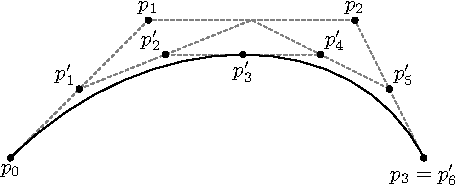
\includegraphics{subdivision}
	     \caption{A Figure}
	 \label{subd}
	\end{figure}

\clearpage %% starts a new page and stops trying to place floats such as tables and figures

\section{More Figure Stuff}
You can also scale and rotate figures.
 	\begin{figure}[h!]
	   
	       \centering
	    % DO NOT ADD A FILENAME EXTENSION TO THE GRAPHIC FILE
	    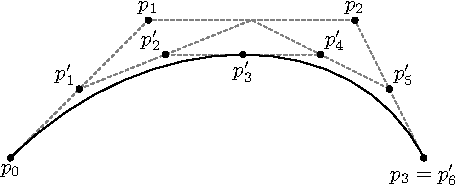
\includegraphics[scale=0.5,angle=180]{subdivision}
	    % if your figure shows up not where you want it, it may just be too big to fit. You can use the scale argument to shrink it, e.g. scale=0.85 is 85 percent of the original size. 
	     \caption{A Smaller Figure, Flipped Upside Down}
	 \label{subd2}
	\end{figure}

\section{Even More Figure Stuff}
With some clever work you can crop a figure, which is handy if (for instance) your EPS or PDF is a little graphic on a whole sheet of paper. The viewport arguments are the lower-left and upper-right coordinates for the area you want to crop.

 	\begin{figure}[h!]
	    	       \centering
	    % DO NOT ADD A FILENAME EXTENSION TO THE GRAPHIC FILE
	   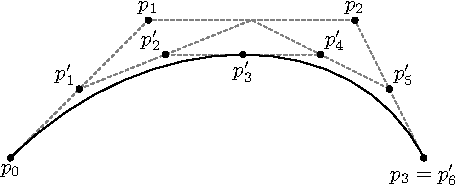
\includegraphics[clip=true, viewport=.0in .0in 1in 1in]{subdivision}
	    \caption{A Cropped Figure}
	 \label{subd3}
	\end{figure}
	
      \subsection{Common Modifications}
      The following figure features the more popular changes thesis students want to their figures. This information is also on the web at \url{web.reed.edu/cis/help/latex/graphics.html}.
    %\renewcommand{\thefigure}{0.\arabic{figure}} 	% Renumbers the figure to the type 0.x
    %\addtocounter{figure}{4} 						% starts the figure numbering at 4
    \begin{figure}[htbp]
    \begin{center}
   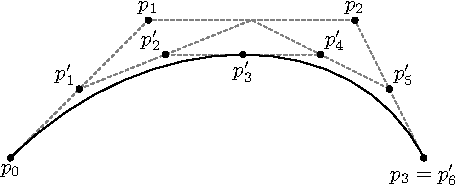
\includegraphics[scale=0.5]{subdivision}
    \caption[Subdivision of arc segments]{\footnotesize{Subdivision of arc segments. You can see that $ p_3 = p_6^\prime$.}} %the special ToC caption is in square brackets. The \footnotesize makes the figure caption smaller
    \label{barplot}
    \end{center}
    \end{figure} 

\chapter*{Conclusion}
         \addcontentsline{toc}{chapter}{Conclusion}
	\chaptermark{Conclusion}
	\markboth{Conclusion}{Conclusion}
	\setcounter{chapter}{4}
	\setcounter{section}{0}
	
Here's a conclusion, demonstrating the use of all that manual incrementing and table of contents adding that has to happen if you use the starred form of the chapter command. The deal is, the chapter command in \LaTeX\ does a lot of things: it increments the chapter counter, it resets the section counter to zero, it puts the name of the chapter into the table of contents and the running headers, and probably some other stuff. 

So, if you remove all that stuff because you don't like it to say ``Chapter 4: Conclusion'', then you have to manually add all the things \LaTeX\ would normally do for you. Maybe someday we'll write a new chapter macro that doesn't add ``Chapter X'' to the beginning of every chapter title.

\section{More info}
And here's some other random info: the first paragraph after a chapter title or section head \emph{shouldn't be} indented, because indents are to tell the reader that you're starting a new paragraph. Since that's obvious after a chapter or section title, proper typesetting doesn't add an indent there. 


%If you feel it necessary to include an appendix, it goes here.
    \appendix
      \chapter{The First Appendix}
      \chapter{The Second Appendix, for Fun}


%This is where endnotes are supposed to go, if you have them.
%I have no idea how endnotes work with LaTeX.

  \backmatter % backmatter makes the index and bibliography appear properly in the t.o.c...

% if you're using bibtex, the next line forces every entry in the bibtex file to be included
% in your bibliography, regardless of whether or not you've cited it in the thesis.
    \nocite{*}

% Rename my bibliography to be called "Works Cited" and not "References" or ``Bibliography''
% \renewcommand{\bibname}{Works Cited}

%    \bibliographystyle{bsts/mla-good} % there are a variety of styles available; 
%  \bibliographystyle{plainnat}
% replace ``plainnat'' with the style of choice. You can refer to files in the bsts or APA 
% subfolder, e.g. 
 \bibliographystyle{APA/apa-good}  % or
 \bibliography{thesis}
 % Comment the above two lines and uncomment the next line to use biblatex-chicago.
 %\printbibliography[heading=bibintoc]

% Finally, an index would go here... but it is also optional.
\end{document}
